\subsection{Quicksort mit Three-Way-Partitioning}

Bei dieser Variante von Quicksort handelt es sich um eine Implementierung von \textit{Robert Sedgewick} und \textit{Jon Bentey}\footnote{siehe: https://www.cs.princeton.edu/~rs/talks/QuicksortIsOptimal.pdf}. Bei dieser Variante werden drei Partitionen erstellt, die Erste enthält Elemente, die kleiner sind als das Pivotelement, die Zweite alle Elemente, welche gleich groß sind wie das Pivotelement und die letzte Partition enthält die  Größeren.

\begin{figure}[htbp] 
	\centering
	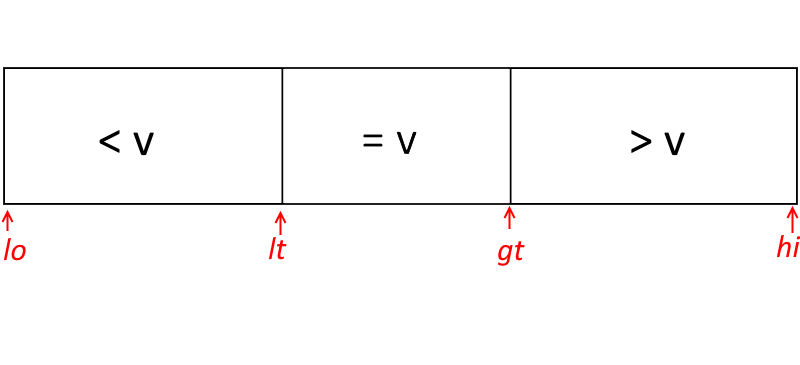
\includegraphics[width=0.5\textwidth]{./img/quicksort-threeway}
	\caption{Quicksort mit drei Partitionen.}
\end{figure}

\noindent
Zwei Variablen $i$ und $j$ laufen vom Anfang beziehungsweise dem Ende des Arrays aufeinander zu und verteilen die Elemente bezüglich des Pivotelementes . Wenn die Zeiger sich überschneiden entstehen zwei Teilmengen, welche anschließend rekursiv mit Quicksort sortiert werden. Dies wiederholt sich, bis schließlich das komplette Array sortiert vorliegt.

Quicksort hat eine Komplexität von $O(n*log(n))$ im besten und durchschnittlichen Fall sowie eine Komplexität von $O(n^2)$ im schlechtesten. Die Laufzeit hängt im Wesentlichen von der Wahl des Pivotelementes  ab, liegt dieses beispielsweise am Ende oder Anfang des Arrays wird jeder Rekursionsschritt nur um eins keiner, was dem schlechtesten Fall entspricht.\\

\newpage

\noindent
\textbf{Beispiel 3.5.1 - Ausführung von Quicksort Three-Way-Partitioning}

\noindent
Für das Beispiel werden die in Abbildung 2 gezeigten variablen $lo$, $lt$, $gt$ und $hi$ verwendet. Ein Zeiger $i = lo$ startet von Beginn des Arrays und wandert bis an das Ende. Als Pivotelement $p$ wird die Mitte des Arrays verwendet (blau hervorgehoben). Der Algorithmus startet also mit:
\begin{gather*}
	A := \{4, 15, 9, 1, \textcolor{blue}{7}, 10, 9, 1, 2, 5\},\; p=7
\end{gather*}
\noindent
Während der Zeiger $i$ von links nach rechts wandert werden für jede Stelle im Array folgende Prüfungen angewendet.
\begin{itemize}
	\item Wenn $A[i] < p$ tausche $A[lt]$ und $A[i]$, anschließend inkrementiere $lt$ und $i$.
	\item Wenn $A[i] > p$ tausche $A[i]$ und $A[gt]$, anschließend dekrementiere $gt$.
	\item Wenn $A[i] = p$ inkrementiere $i$.
\end{itemize}